\section{Design Overview}


Our goal is to design a bi-directional VLC system that runs on battery-free devices like smartphones and sensor nodes. The system features an LED and a mobile device. One closed-loop communication paradigm of the system is as follows. The LED sends a packet carried on the white light it emits modulated to $1MHz$ (downlink). The \vitag\ senses the transmission and wakes up. Upon successfully receiving and demodulating the packet, the \vitag\ sends a packet back to the LED (uplink). The LED is slightly modified so as to integrate the receiver in as shown in Fig. \ref{system}.

In sending the packet, instead of generating the signal using power-consuming LEDs or other communication channels such as infrared or ultraviolet carriers, we adopt the modulating retro-reflector framework, with the combination of an LCD and a retro-reflector. Driving the LCD costs only \hl{xx $\mu W$} energy. In addition, a \vitag\ passively sends signals, thus the power consumption of which can be maintained at a low level. 

%with the help from other energy saving components. Finally,  The receiver detects any signals sent by the \vitag, and decodes the bits against noises and interferences.

In the rest of the paper, we describe the design of \retro\ that consists of a modified off-the-shelf white LED and a \vitag\ in more details.

\p{We need a system architecture figure here}

\begin{figure}[th]
   \centering
   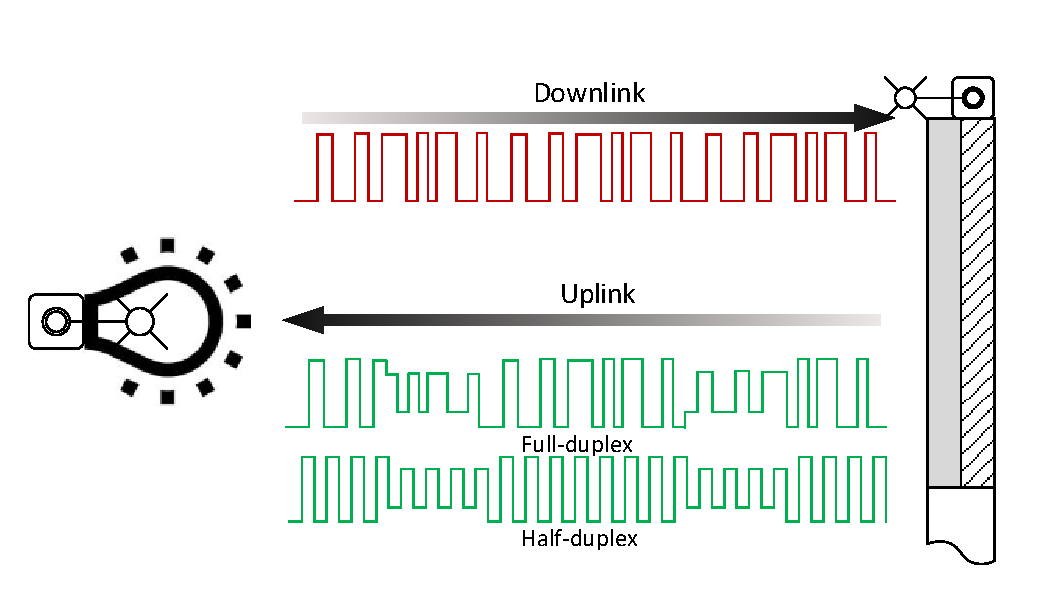
\includegraphics[width=0.8\columnwidth]{link.pdf}
   \caption{Downlink and uplink.}
   \label{fig:link}
   \vskip -3mm
\end{figure}

% Our goal is to design primitives that enhance visible light communication capabilities on battery-free devices while preserving user privacy and security of both the transmitters and the receivers, with the omnipresence of readily available LEDs that serve as the lightening devices. The key challenge in achieving these is two-fold. First, devices running at visible light bands are power-intensive because of the broad bandwidth these bands can provide. Second, the noise caused by ambient signals on the visible light spectrum and the interference triggered by the the data transmitted by the system itself stays in the same band as what the receiver expects to receive at. To address these challenges, we use the following guiding principles: we use as many analog components and recycle as much energy as possible on the tag to enable the tag to transmit to the reader with a decent data rate. Also, we diminish the scattering area as much as possible by making use of directional backscattering materials of small Field of View (FoV). Such approaches, as we show in the rest of the paper, can provide an order of magnitude reduction in the power consumption of these communication primitives and in the scattering area of the signals on the backscattering channel.

% In the rest of this paper, we describe \vitag, our battery-free tag and show how it can enable backscatter communications with no battery and with a higher energy efficiency with respect to communication range than tags with LEDs on. We then describe \reader, our system that can be easily integrated onto commercial LED lights for transmitting data at no discernible flickers with dimming support and receiving with \hl{hhh dB} signal-to-interference-plus-noise-ratio (SINR). Finally, we show that our designs can be used to enable concurrent transmissions in a network of battery-free devices without the need for synchronization.